\chapter{LitQEval}\label{ch:ownApproach}
Despite ongoing research on automatic literature query generation and related evaluations with medical datasets, such as CLEF \autocite{kanoulas2017clef, kanoulas2018clef, kanoulas2019clef} and the Collection of Seeds \autocite{Wang_2022}, the insights gained from these evaluation metrics are not particularly compelling for our use case. This limitation arises from two main factors. 

First, the CLEF and Collection of Seeds datasets are exclusively focused on medical data. Although Badami's work \autocite{badami2023adaptive} offers a more diverse dataset, it lacks a suitable evaluation metric. Their evaluation primarily aims to maximize recall, with minimal consideration for precision, as literature search queries often yield far more results than necessary, making precision a less effective measure in this context. 

A second limitation arises when recall is prioritized exclusively. For example, if we aim to train a model to generate queries that maximize recall, there is no penalty for generating overly broad queries, such as those that exploit wildcards, which could lead to an excessive number of irrelevant results.

To address these issues, we introduce a dataset structured similarly to that of Badami \autocite{badami2023adaptive} but designed to be more comprehensive and covering a wider range of topics. Alongside this dataset, we propose new evaluation metrics that account for the inherently broad nature of literature search queries while penalizing excessively large queries. These metrics also emphasize the importance of accurately identifying core publications that are deemed highly relevant within the domain.


\section{Dataset}
The dataset we aim to create has two primary goals: First, it should encompass a wide range of randomly selected scientific research fields. Second, for each selected field, it should contain a set of highly relevant publications to serve as anchors for evaluating additional publications found in these areas.

Selecting new research topics is straightforward; however, to avoid bias from ongoing research interests, we used ChatGPT to generate a list of scientific fields that are recent and not overly broad. For instance, a topic like \textit{Artificial Intelligence} is vast, making it challenging to accurately and comprehensively identify core publications. Instead, we chose a more specific, problem-focused topics such as \textit{Drones in Agriculture}. To search for the corresponding bibliometric analysis we used the following query: \textit{<TERM>  ("Bibliometric" OR "Scientometric" OR "Systematic literature" OR "Most Influential" OR "Most Cited" OR "Scientific Landscape" OR "Literature Landscape" OR "Core Literature")} 


After identifying a sufficient number of diverse fields, 15 in our case, we sought to collect core publications for each field. Due to the difficulty of gathering core publications across a broad array of topics, we leveraged the bibliometrics community’s expertise. Specifically, we searched for bibliometric studies that identify the most relevant publications within each research area. For example, a bibliometric analysis of \textit{Drones in Agriculture} \autocite{Rejeb2022} lists the most cited publications from 1990 to 2021. In this case, 40 core publications were identified, which we manually located on Dimensions.ai and added to our dataset, omitting any publications not found in Dimensions.

This process was repeated across all selected research fields, resulting in a dataset containing 15 topics, each with 25–50 core publications, as illustrated in \autoref{fig:dataset-overview}.
\begin{figure}
	\centering	
	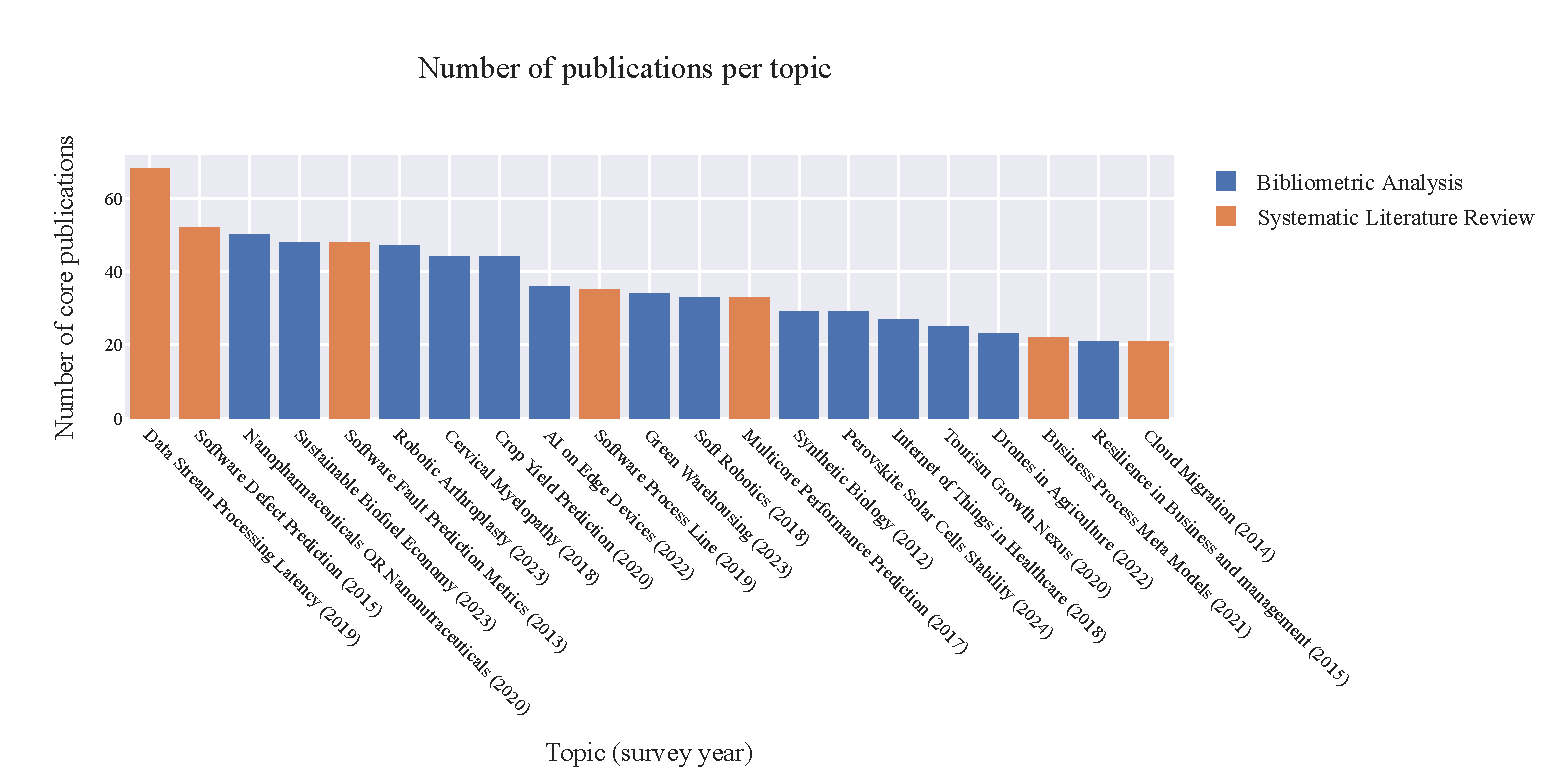
\includegraphics{pics/dataset-overview.pdf}
	\caption[Dataset overview of the research topics]{An overview of the dataset and the selected 15 research fields with respective core publications identified through bibliometric analyses. The number in brackets following the field name on the x-axis represents the year of the analysis.}
	\label{fig:dataset-overview}
\end{figure}


\subsection{Dataset Analysis}
We recognize that potential biases may exist in our dataset due to its complete reliance on the bibliometric community for identifying core publications. This often implies that publications with higher citation counts are deemed more relevant. To assess this, we analyzed the citation distribution per topic, as provided by Dimensions, shown in \autoref{fig:dataset-citation}. Additionally, we examined the distribution of publication years per topic, illustrating the time span considered in the bibliometric analyses, as shown in \autoref{fig:dataset-years}.  If we compare the distribution of publication years for the medical research field \textit{Cervical Myelopathy} with that of \textit{IoT in Healthcare}, both of which were published in 2018, we can observe distinct differences in the year distributions of their core publications. These variations may be attributed to factors such as the recency of the field, changes in terminology over time, or the nature of the research area, where one field may prioritize more established works while the other focuses on recent advancements.

For the evaluation pipeline that we will introduce, the embeddings of the core documents are essential for effectively assessing the search query, as detailed in \autoref{sec:eval-metrics}. To validate this approach, we examine the clustered embeddings of the titles and abstracts for each core topic, as well as the bibliometric analyses in which these documents were initially referenced. This enables us to assess whether core publications within each field exhibit semantic similarity while also demonstrating some degree of dissimilarity from publications in other topics. The resulting clusters, shown in \autoref{fig:dataset-clustering}, were generated using k-means clustering, where $k$ is set to the number of topics. For this, we use OpenAI's small embeddings model alongside t-SNE\autocite{van2008visualizing} to reduce the dimensionality of the non-linear embedding vectors to two dimensions.


\begin{figure}[!hb]
	\centering	
	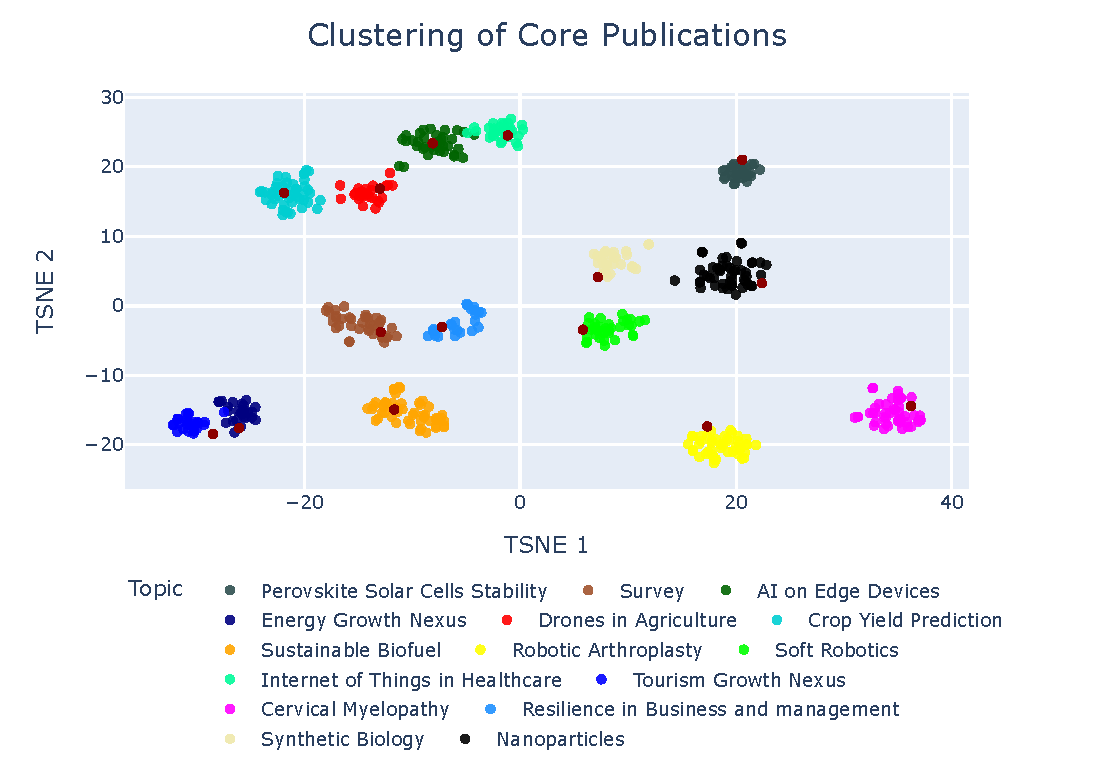
\includegraphics[scale=0.4]{pics/tnse_clustering.pdf}
		\caption[Core Publications Clustering]{This illustration shows a clustering of publication embeddings generated using the titles and abstracts of each corresponding publication. These were embedded using OpenAI's small embedding model, with t-SNE applied to reduce the high dimensionality of the embeddings. The results were then clustered using k-means, where $k$ is set to 15 (representing the number of topics). The clustering effectively groups core publications within each field based on semantic similarity. Exceptions include \textit{IoT in Healthcare} and \textit{AI on Edge Devices}, as well as \textit{Tourism Growth Nexus} and \textit{Energy Growth Nexus}, which overlap due to the inherent similarity in the respective literature.}
	\label{fig:dataset-clustering}
\end{figure}

 
\section{Evaluation metrics}\label{sec:eval-metrics}
\lipsum[1-3]
